%% LyX 2.1.4 created this file.  For more info, see http://www.lyx.org/.
%% Do not edit unless you really know what you are doing.
\documentclass[english]{article}
\usepackage[T1]{fontenc}
\usepackage[latin9]{inputenc}
\usepackage{graphicx}

\makeatletter
%%%%%%%%%%%%%%%%%%%%%%%%%%%%%% User specified LaTeX commands.
%% This document created by Scientific Word (R) Version 3.0




\usepackage{amsfonts}


%TCIDATA{OutputFilter=latex2.dll}
%TCIDATA{CSTFile=LaTeX article (bright).cst}
%TCIDATA{Created=Mon Nov 24 12:24:47 2003}
%TCIDATA{LastRevised=Fri Nov 28 11:39:52 2003}
%TCIDATA{<META NAME="GraphicsSave" CONTENT="32">}
%TCIDATA{<META NAME="DocumentShell" CONTENT="General\Blank Document">}
%TCIDATA{Language=American English}
\newtheorem{theorem}{Theorem}
\newtheorem{acknowledgement}[theorem]{Acknowledgement}
\newtheorem{algorithm}[theorem]{Algorithm}
\newtheorem{axiom}[theorem]{Axiom}
\newtheorem{case}[theorem]{Case}
\newtheorem{claim}[theorem]{Claim}
\newtheorem{conclusion}[theorem]{Conclusion}
\newtheorem{condition}[theorem]{Condition}
\newtheorem{conjecture}[theorem]{Conjecture}
\newtheorem{corollary}[theorem]{Corollary}
\newtheorem{criterion}[theorem]{Criterion}
\newtheorem{definition}[theorem]{Definition}
\newtheorem{example}[theorem]{Example}
\newtheorem{exercise}[theorem]{Exercise}
\newtheorem{lemma}[theorem]{Lemma}
\newtheorem{notation}[theorem]{Notation}
\newtheorem{problem}[theorem]{Problem}
\newtheorem{proposition}[theorem]{Proposition}
\newtheorem{remark}[theorem]{Remark}
\newtheorem{solution}[theorem]{Solution}
\newtheorem{summary}[theorem]{Summary}
\newenvironment{proof}[1][Proof]{\textbf{#1.} }{\ \rule{0.5em}{0.5em}}

\makeatother

\usepackage{babel}
\begin{document}

\title{Public Goods}


\author{Michael Peters}


\date{\today}

\maketitle

\section{Introduction}

In this reading, a \emph{public good} is one having the property that
once it has been produced, it can be made freely available to everyone.
An mp3 file, or a computer program would fit into this category. Contrast
this with the \emph{private goods} we have discussed so far. If one
person consumes a private good, no other consumer can have that good.
Some of the more important goods in the modern economics are actually
public in this sense. For example, an idea or a bit of information
is a public good. Whether or not you know the idea, or have the information
does not impact on my ability to know the same thing or have the same
information (though whether or not you have the same information as
I do may determine whether or not I can make money off you). A music
file shared on my computer is a public good -- if you download it
from my website, my ability to enjoy it is not affected at all. A
theorem, like the first welfare theorem that we studied last week,
is a public good: I do not forget it when you learn it. Contrast this
with my car or my lunch which are both private goods: if you take
them from me I cannot enjoy them at all.

This note describes an equilibrium for the \emph{voluntary contribution
game}, which is a common way to think about how public goods are provided.
It explains why the amount of the public good in the voluntary contribution
game is under produced (because the outcome is not Pareto optimal:
there is another outcome that will make everyone better off). 


\subsection{The voluntary contribution game}

Suppose there are two goods, one public ($y$) and one private ($x$).
Let $f\left(x\right)$ denote the amount of the public good that can
be produced from $x$ units of the private good. Suppose there are
two consumers with utility functions $u_{1}\left(x,y\right)$ and
$u_{2}\left(x,y\right)$ respectively. Their endowments of the private
good are $\omega_{1}$ and $\omega_{2}$. The set of points $\left\{ \left(x,y\right):y=f\left(\omega_{1}+\omega_{2}-x\right)\right\} $
is the \emph{production possibilities frontier}.

If the first consumer decides to consume $x_{1}$ (and devote the
rest of his endowment $\omega_{1}$ to production of the public good)
while consumer $2$ decides to consume $x_{2}$ the utilities of each
of the consumers are given by
\[
u_{1}\left(x_{1},f\left(\omega_{1}+\omega_{2}-x_{1}-x_{2}\right)\right)
\]
 for consumer $1$ and
\[
u_{2}\left(x_{2},f\left(\omega_{1}+\omega_{2}-x_{1}-x_{2}\right)\right)
\]
 for consumer $2$. The important point is that if consumer $1$,
say, decides to consume a bit less of the private good and produce
a bit more of the public good, then consumer $2$ will enjoy the additional
public good too without any cost at all.

The voluntary contribution game equilibrium is one way to predict
how much of the private good each consumer will choose. Each of the
consumers simply picks the amount of the private good they want on
their own. This is a bit hard to do because the amount that each consumer
will choose to contribute depends on how much they expect the other
consumer to contribute. A good way to do this is to use a \emph{Nash
equilibrium} in place of a Walrasian equilibrium. Instead of taking
prices to be fixed, each consumer takes the contribution of the other
consumer to be fixed and chooses the contribution that maximizes his
utility given this expectation. In a Walrasian equilibrium, when a
consumer acts as if he believes that prices are fixed, he has to be
physically able to purchase the bundle that maximizes his utility
at these prices. That is why the price expectations have to be such
that markets clear. Analogously, when the consumer chooses his optimal
contribution given a fixed expectation about the contribution of the
other consumer, he has to end up with exactly the amount of the public
good that he expected to get.

Formally, a Nash equilibrium for the voluntary contribution game is
a pair of private consumptions $x_{1}^{\ast}$ and $x_{2}^{\ast}$
such that
\begin{equation}
u_{1}\left(x_{1}^{\ast},f\left(\omega_{1}+\omega_{2}-x_{1}^{\ast}-x_{2}^{\ast}\right)\right)\geq u_{1}\left(x^{\prime},f\left(\omega_{1}+\omega_{2}-x^{\prime}-x_{2}^{\ast}\right)\right)\label{consumer_1}
\end{equation}
 for any alternative contribution $x^{\prime}\in\left[0,\omega_{1}\right]$
and
\begin{equation}
u_{2}\left(x_{2}^{\ast},f\left(\omega_{1}+\omega_{2}-x_{1}^{\ast}-x_{2}^{\ast}\right)\right)\geq u_{2}\left(x^{\prime},f\left(\omega_{1}+\omega_{2}-x_{1}^{\ast}-x^{\prime}\right)\right)\label{consumer_2}
\end{equation}
 for any alternative contribution $x^{\prime}\in\left[0,\omega_{2}\right]$.

One way to view the outcome of this game is given in Figure $1$ where
the two consumers choose $x_{1}^{\ast}$ and $x_{2}^{\ast}$. The
`budget line' that consumer $1$ faces, for example, when consumer
$2$ chooses consumption $x_{2}^{\ast}$ is the set of all pairs $\left\{ \left(x_{1},y\right):y=f\left(\omega_{1}+\omega_{2}-x_{1}-x_{2}^{\ast}\right)\right\} $.
The slope of this is exactly the same as the slope of the production
possibilities frontier at the point $\left(x_{1}^{\ast}+x_{2}^{\ast},y^{\ast}\right)$.
The same is true for consumer $2$. So, in the equilibrium of the
voluntary contribution game, each consumer has the same marginal rate
of substitution and the same marginal rate of transformation in production.

\begin{center}
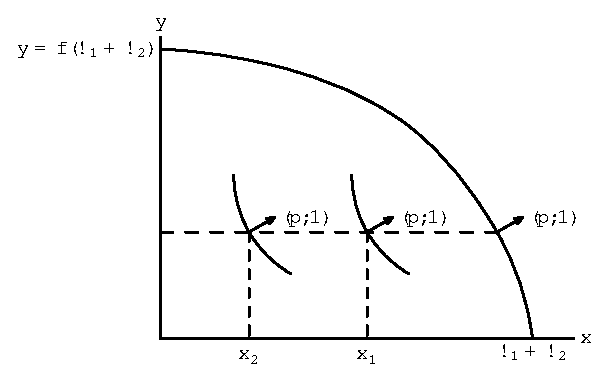
\includegraphics{public_goods_fig1}
\par\end{center}

With private goods, this is exactly what you want. Recall that, in
the Edgeworth box, both consumers' indifference curves were tangent
and the common slope of their indifference curves was equal to the
slope of the production possibilities frontier. With public goods,
this is not the outcome that you want.

An alternative approach -- that helps to explain how contributions
are determined and why these contributions are not Pareto optimal
-- is to try find the best choice for consumer $1$ to make for all
the different possible contribution levels that consumer $2$ might
choose. This approach is more common in game theory and involves the
construction of something called the \emph{best reply function}. The
best reply functions are put together to understand the final outcome.

In Figure 2, the various \emph{consumption choices} that player $2$
can make are given along the bottom axis. Each such choice implies
a contribution to the production of the public good - just take the
difference between the consumption level and the endowment to find
it.

\begin{center}
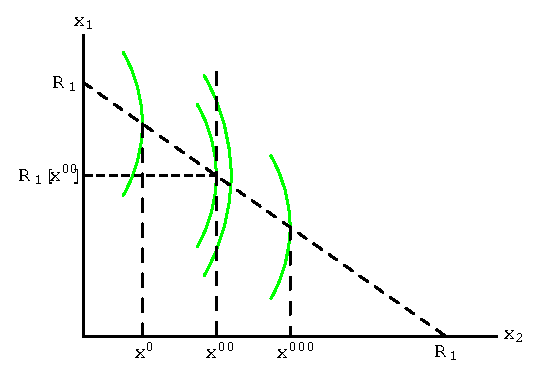
\includegraphics[width=3.5414in,height=2.399in]{public_goods_fig2}
\par\end{center}

The green lines represent iso-utility curves for consumer $1$. They
are solutions to equations of the form
\[
u_{1}\left(x_{1},f\left(\omega_{1}+\omega_{2}-x_{1}-x_{2}\right)\right)=K
\]
 where $K$ is some constant. Consumer $1$ achieves higher utility
(holding his own consumption level constant) the \emph{lower} is the
consumption level of consumer $2$. Lower consumption by consumer
$2$ means that consumer $2$ is contributing more of her endowment
to produce the public good.

In the Nash equilibrium, consumer $1$ forms some belief about the
consumption level that consumer $2$ will pick. Suppose for the moment,
that he believes that consumer $2$ will choose consumption $x^{\prime\prime}$.
Then he can attain any $\left(x_{1},x_{2}\right)$ combination that
lies on the vertical line through $x^{\prime\prime}$. The best such
point is the one that lies on the highest iso-utility curve. That
is the one through the point $\left(R_{1}\left[x^{\prime\prime}\right],x^{\prime\prime}\right)$
where an iso-utility curve is just tangent to this vertical line.
(If he were to lower his planned consumption by moving down this vertical
line, he would end up on a lower iso-utility curve like the one that
lies just to the right of the point $\left(R_{1}\left[x^{\prime\prime}\right],x^{\prime\prime}\right)$.

There would be a different best choice like this for every different
choice that consumer $2$ makes. The picture shows the corresponding
tangencies at point $x^{\prime}$ and $x^{\prime\prime\prime}$. If
you joined all these best choices together they would form a line
(not necessarily straight as it is in the picture) called consumer
$1$'s reaction function. This is the line $R_{1}R_{1}$ in the picture.
It explains what consumer $1$ would choose to do for every possible
different belief that he might have about the consumption choice of
consumer $2$.

\begin{center}
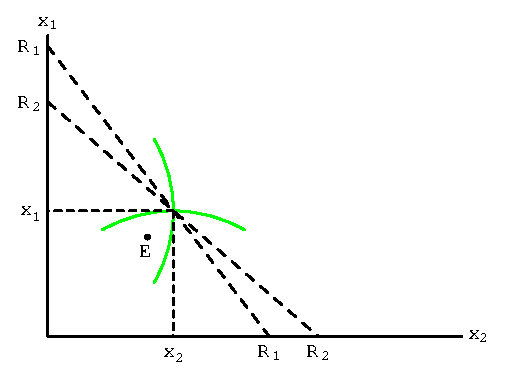
\includegraphics[width=3.2949in,height=2.412in]{public_goods_fig3}
\par\end{center}

Doing the same exercise for consumer $2$ yields a similar curve,
which is drawn in Figure $3$ as $R_{2}R_{2}$. The point where these
two curves intersect is the Nash equilibrium. Each consumer chooses
his best consumption given what he expects the other consumer to choose;
and, as it turns out, the other consumer always does exactly what
he expects him to do.

When you try to construct the iso-utility curves for person $2$,
he will choose one that is tangent to the flat line through $x_{1}^{\ast}$
since he expects consumer $1$'s consumption choice to be $x_{1}^{\ast}$
no matter what he does. This means that the iso-utility curves for
the two consumers must cut through each other as shown in the diagram.
There must be a point like $E$ where both of the consumers would
be better off if they could jointly agree to move there. That would
involve each of them reducing their own consumption of the private
good and using that to increase production of the public good.


\section{What is wrong with the outcome in the voluntary contribution game.}

Since it is so important to understand how externalities work in economics,
lets make the argument in a different way. This exercise also helps
to understand the methods that micro economists sometimes use to describe
why institutions work badly, and the sorts of ideas they propose to
fix them.

To begin, lets revert to the picture we have used so far to describe
allocations, with the total consumption of the private good on the
horizontal axis and the output of the putblic good on the vertical
axis. For the purposes of this argument, lets just imagine that the
private good is money. The public good is any good that can be reproduced
at zero marginal cost. I'll call it software.

Typical software programs use existing libraries to carry out simple
tasks that come about during the creation of some higher level process.
For example, a web page that displays an ad may request the ad from
some other computer on a network. The 'process' of requesting an ad
or any bit of infomration over a network in the course of building
a webpage is patentable. The actual code that carries out the request
is a software program that is subject copyright - two different levels
of protection. If there is no patent on the process, then the copyright
holder can prevent someone else from using his or her program to make
a network request unless they pay a fee. If you aren't willing to
pay the fee, then you can write your own version of the program. If
the \emph{process }of making a network request is also patented, then
you can't actually make a network request without paying a fee.

In Canada and the US, patents have nothing to do with invention, the
first person to apply for a patent gets it no matter who 'invented',
if that is the right word, the process. In many ways the reason that
companies apply for patents is to protect themselves from other patent
holders. If they have a patent \emph{portfolio }then they can make
cross licensing agreements with other large companies that also have
portfolios. These agreements mean that the companies agree not to
sue each other for patent infringement. The sort of companies that
make these agreements -- Microsoft, Apple, Dell, Samsung. Of course,
this creates an even bigger pool of patents these companies can use
to sue other entrants.

What has saved the tech sector from software patents is open source
software -- Google, Facebook and the other big social media giants
have been developed using open source software. At least in my experience,
they tend to give back by giving their own code open source licenses
so that other firms can use it.

In the story that follows software means the bundles of library code
and software methods that users develop to carry out their day to
day activities over the computer. Each of the two consumers below
writes software for this purpose. The voluntary contribution game
approximates the open source method. We'll try to compare that with
what happens in the patent sector.

As in the voluntary contribution story given above, each consumer
has a payoff $u_{i}\left(x,y\right)$ that depends on $x$, the amount
of their money income they keep for themselves, and $y$ the total
amount of software code that they use. The software is freely redistributable
since an essentially unlimited number of copies of the software can
be made at no extra cost, so it satisfies the definition of a public
good as we described it above. Indifference curves for consumer 1
are bundles that give him or her the same level of utility. For consumer
1, this is really straightforward. The indifference curve is just
the collection of $\left(x,y\right)$ pairs that satisfy
\[
u_{1}\left(x,y\right)=K.
\]
The graphs of these curves look no different than they do in any other
problem. Higher indifference curves (further away from the origin)
represent higher values of $K$ in the equation above, and correspondingly
higher payoffs to consumers. 

The leap we are going to make here is that when we choose a bundle
$\left(x,y\right)$ for consumer 1, this bundle induces a corresponding
bundle for consumer 2 given by
\[
\left(\omega_{1}+\omega_{2}-f^{-1}\left(y\right)-x,y\right).
\]
In words, we figure out how much money is required to produce $y$,
that is the $f^{-1}\left(y\right)$, then subtract that from the total
endowment $\omega_{1}+\omega_{2}$ to get the total amount of money
left over after producing $y$ units of software. Subtract the $x$
we want to give to consumer 1, then give the rest to consumer 2. The
function $f^{-1}\left(y\right)$ is sometimes referred to as the cost
function for the public good.

Given this logic, we could define an indifference curve for \emph{consumer
2 }by finding all the consumption bundles for \emph{consumer 1 }that
induce the same payoff for player 2. Formally, an indifference curve
for player 2 is the collection of all bundles for player 1 that satisfy
\[
u_{2}\left(\omega_{1}+\omega_{2}-f^{-1}\left(y\right)-x,y\right)=K.
\]
\emph{ }To figure out what these indifference curves look like is
a bit daunting. Holding $y$ constant, the less money consumer 1 has,
the more is left over for consumer 2. In this sense, player 2's indifference
curves represent higher payoffs for 2 the closer they are to the origin. 

For the rest, we'll rely on the idea that the public good provides
diminishing marginal utility to consumer 2. What that means is that
the more of the public good that is being produced, the less valuable
an additional unit of the public good will be. Fix the consumption
of the private good of consumer 1 at some value $x_{0}$ and travel
up the vertical line through $x_{0}$. Remember that changing the
public good in this case means that all the cost of producing the
public good is borne by consumer 2 since the amount of money consumer
1 has is being held constant at $x_{0}$. Initially as you increase
the public good, this makes consumer 2 better off since the public
good is very valuable to her when there isn't much of it. Eventually
the thrill will wear off, and as the production of the public good
gets higher and higher, consumer 2's payoff will begin to decline.
What that means is that consumer 2's indifference curves will typically
cross any vertical line twice.

Of course, there will be one indifference curve that is just tangent
to the vertical line. This one is illustrated in the picture below. 

The indifference curves should look like backward C's as in the following
diagram, where I have superimposed consumer 2's indifference curve
into the original diagram depicting the Nash equilibrium of the voluntary
contribution game. Let me explain why. At the point where the indifference
curve is just tangent to the vertical line, consumer 2 could increase
her production of software $y$ and travel further up the vertical
line. If she travels directly upward, it means that she is holding
consumer 1's holdings of money constant. In other words, if she increases
production, she pays all the costs herself. At the tangency, she doesn't
want to do this - the marginal benefit she gets from increasing production
is exactly equal to the marginal cost. Formally
\[
\frac{\partial u_{2}\left(\omega_{1}+\omega_{2}-f^{-1}\left(y^{\ast}\right)-x_{1}^{\ast},y^{\ast}\right)}{\partial x}\frac{1}{f^{\prime}\left(y^{\ast}\right)}=\frac{\partial u_{2}\left(\omega_{1}+\omega_{2}-f^{-1}\left(y^{\ast}\right)-x_{1}^{\ast},y^{\ast}\right)}{\partial y}.
\]


Then if you travel up the vertical line a bit above $\left(x_{1}^{\ast},y^{\ast}\right)$,
then consumer 2 is strictly worse off. How to restore her payoff?
You have to give her more money, which means reducing the amount of
money you leave for consumer 1. That means that you have to travel
left of the vertical line to restore 2's payoff. The indifference
curve must lie to the left of the vertical line at every point except
at the tangency.

\begin{center}
\includegraphics{public_goods_fig5}
\par\end{center}

Since the point $\left(x_{1}^{\ast},y^{\ast}\right)$ is supposed
to coincide with the Nash equilibrium in the voluntary contribution
game, consumer 1's indifference curve has the same slope as the production
possibilities frontier at the point where $y^{\ast}$ is produced.
In other words, it is downward sloping, not vertical. The lens between
the curves represents a situation in which both consumers could be
made better off - same thing we showed above.

Theoretically, in an open source software world, too little software
will be produced. 


\section{Patents}

In real life, the fact that an outcome isn't pareto optimal doesn't
necessarily make it bad. As I mentioned above, the software products
you probably use the most, Google search, Facebook and Twitter all
use opensource software and give back a bunch of the code they write.
The programming languages which drive most web pages, php, python,
and javascript, are all open source.

Thanks to good old fashioned economic theory, the fact that the equilibrium
of the voluntary contribution game is not pareto optimal makes it
sound like this is a problem and that SOMETHING MUST BE DONE! Big
corporations have lots of talented people working for them and this
gave them an idea. Patents are 'something' therefore WE MUST HAVE
PATENTS.

You can read about US copyright and patent laws in a lovely (free)
book called ``Against Intellectual Monopoly'' by David Levine and
Michele Boldrin (http://www.dklevine.com/general/intellectual/againstfinal.htm).
The book is full of historical anecdotes and simple economic models
to explain what is going on. The gist of their argument is that copyright
and patent laws in the US are designed to give corporations levers
that they can use to prevent entry and suppress competition. Evidence
that these laws encourage creation of public goods is basically non-existent,
what evidence there is suggests the opposite. This is important for
Canada since the US almost always insists that countries adopt US
copyright and patent law before they will engage in trade negotiation.

The way patents work is that one of the two consumers applies for
a patent, and is then given a monopoly over production of the patented
product, in this case our software. As I mentioned above, the US (and
now Canada) has what is called a 'First to Patent' law, which means
that whoever files a patent on something first gets the patent whether
they developed the idea or not. This creates its own problems. For
example, patents are sometimes granted after methods are being widely
used - one click shopping, and dynamic pricing being examples. Lets
ignore this, and just suppose consumer 2 wins this race. Consumer
2 now owns the public good, and can charge whatever price she likes
for it. Suppose she sets the price $p$ for the public good.

Normally we do all our stuff using the price of good $x$ and letting
the price of good 1 be normalized to 1. We'll switch that here, but
this shouldn't create too much of a problem. The public good $y$
has a price $p$ , while the private good has price 1. Given the price
set by consumer 2, consumer 1 now finds the best bundle of public
and private goods he can afford. This is given by the point where
his indifference curve is tangent to the budget line that passes through
the point $\left(\omega_{1},0\right)$. Why care? The reason is that
consumer 1 will no longer be able to produce the public good on his
own (of if he does, he will have to pay consumer 2 a fee because she
owns the public good). So the price that consumer 2 sets will change
consumer 1's desire to have the public good. If consumer 2 sets a
price too high, consumer 1 won't want any.

What this means is that the patent doesn't by itself give consumer
2 any incentive to produce more of the public good - production depends
on price, which is chosen by consumer 2. What the patent does give
her is a device that she can use to extract money from consumer 1.

The figure below depicts what consumer 1 would want for three different
prices.

\begin{center}
\includegraphics{public_goods_fig6}
\par\end{center}

The steepest budget line is the one that has the lowest price for
the public good, the flattest budget line has the highest price. Since
2 now has the 'intellectual' monopoly, she can set any price that
she likes. She will pick the price that maximizes her payoff. 

It would seem quite daunting to find this price, since the change
in price will change consumer 1's consumption of the public good,
which will in turn effect how much consumer 2 needs to produce. 

Fortunately we have just the graphic device we need figure out what
consumer 2 will do, since we just figured out what her indifference
curves looked like in the space depicting consumer 1's consumption
of the private and public good. She will pick the price that put her
on the highest indifference curve consistent with consumer 1 maximizing
subject to his budget constraint. You'll notice in the curve above
that there is a smooth line that connects all the tangency points
for different prices. This curve is sometimes referred to as the offer
curve. The picture that follows shows what happens when consumer 2
chooses the point on this offer curve that is tangent to her own indifference
curve.

\begin{center}
\includegraphics{public_goods_fig7}
\par\end{center}

The indifference curve for consumer 2 is now tangent to consumer 1's
offer curve so consumer 2 is getting the best payoff she can get.
Consumer 1 is getting the best payoff he can afford. Notice that because
of the way the offer curve is drawn the two consumers indifference
curves won't be tangent. Both consumers would be better off if more
of the public good were produced. So the patent solution just produces
another inefficient outcome. This is why proponents of patents will
never talk about how well patents work. Instead they focus on how
bad the outcome is likely to be without them - we went over that -
not really so bad.

We can continue with graphic reasoning a bit more, but then we'll
need to switch to algebra. The following figure reproduces the outcome
for consumer 1 in the equilibrium of the voluntary contribution game.

\begin{center}
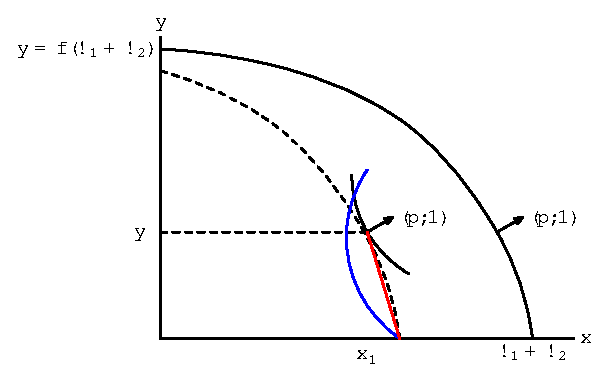
\includegraphics{public_goods_fig9}
\par\end{center}

Recall that the budget line for consumer 1 with patents starts at
his or her endowment point $\left(0,\omega_{1}\right)$. If consumer
2 sets a price for software which allows consumer 1 to buy the outcome
he enjoyed in the volunary contribution game, then the budget line
consumer 1 faces would be given by the red line in the picture. Since
this budget line always lies below the production possibilities curve
that consumer 1 faces in the volutary contribution game, it will be
steeper than consumer 1's indifference curve at his allocation in
the equilibrium of that game.

So far, this is completely working. If the price of the software were
set so that consumer 1 could reproduce the outcome in the volunary
contribution game, then consumer 1 would be able to purchase the additional
software that he wants from consumer 2. Consumer 2 would in turn be
willing to produce it because she is making more than enough money
to compensate her for her additional cost.

What patents get wrong is what they do next - they give consumer 2
control over price. Most economics students understand at some level
that markets don't work when some market participant can control the
price. In this example, it is easy to see why this is the case. The
patent holder now has a new device for earning money that has nothing
at all to do with having to produce software. It would first occur
to her than since she controls price, she can actually get the same
level of the public good $y^{\ast}$ as in the voluntary contribution
game, while ending up with a lot more money for herself. 

In our formalism, we can use consumer 1's offer curve to understand
this. Since the budget line that consumer 1 faces when the price is
set in such a way that he can choose the equilibrium outcome in the
voluntary contribution game is steeper than his indifference curve
at that point, it means that consumer 1's offer curve cuts the horizontal
line through $y^{\ast}$ at a point to the left of consumer 1's original
equilibrium allocation. The offer curve should look like the solid
blue line in the figure above. So consumer 2 can raise the price of
software until the budget line faced by consumer 1 looks like the
green line in the next figure.

\begin{center}
\includegraphics{public_goods_fig10}
\par\end{center}

If you recall that the definition of the offer curve is all the points
at which consumer 1's indifference curve is tangent to a line that
runs from that point back to the endowment point, consumer 1 will
voluntarily choose $y^{\ast}$ units of software when the price is
set to the green line is the budget line. By allowing consumer to
control of the price, the patent basically creates a subsidy to the
patent holder. 

Consumer 2 might not be satisfied with this subsidy. She has really
embarked at this point on a new venture - surplus extraction. Software
is somewhat secondary at this point and she receives her reward by
manipulating price. It is theoretically possible that she might want
to raise output of software, but as in the figures above, this isn't
her main objective, it is to find the place where her indifference
curve is tangent to consumer 1's indifference curve.

Whether she does or not can be determined by travelling along the
dashed horizontal line to the left of the equilibrium point in the
voluntary contribution game until you reach the offer curve, given
by the solid blue line in the figure above. Since consumer 2 can achieve
any point on the offer curve that she wants, what she does will depend
on what her indifference curve looks like through that point. Generally,
the tangency with the offer curve may involve either more or less
software than in the voluntary contribution game. So patents are as
likely from a theoretical perspective to lower output of software
as they are to raise it.

If this graphical reason is getting too complicated, then we can also
do the argument algebraically. Suppose that each consumer has money
income $\omega$ and that one unit of software costs one dollar to
build. Lets also suppose that the consumers both have Cobb Douglas
utility functions with 
\[
u\left(x,y\right)=x^{\alpha}y^{1-\alpha}.
\]
Consumer $1$ maximizes
\[
x^{\alpha}\left(2\omega-x-x_{2}\right)^{1-\alpha}
\]
where $x_{2}$ is the amount of income consumer 1 expects consumer
2 to retain for herself (which makes her contribution to the production
of software $\omega-x_{2}$). This is done subject to the constraint
that $x\le\omega$. 

The first order condition gives
\[
x=\alpha\left(2\omega-x_{2}\right)
\]
which has a solution between $0$ and $\omega$ provided $2\alpha$
is less than 1 and $x_{2}<\omega$. The symmetric equilibrium for
the voluntary contribution game is then 
\[
x=\frac{2\alpha}{1+\alpha}\omega
\]
 for each of the two players. The total output of software would then
be
\begin{equation}
2\omega-\frac{4\alpha}{1+\alpha}\omega=2\omega\frac{\left(1-\alpha\right)}{1+\alpha}.\label{voluntary-y}
\end{equation}


On the other hand, if 2 has the patent, then as you know, consumer
1 will keep the fraction $\alpha$ of his money income and choose
to buy $\frac{\left(1-\alpha\right)\omega}{p}$ units of the public
good. Since $\frac{2}{1+\alpha}\alpha\omega$ is obviously strictly
larger than $\alpha\omega$ you can see that consumer 1 will have
a lot less income with patents. 

So when 2 charges $p$ for the public good, her payoff is
\[
\left(\omega\left(2-\alpha\right)-\frac{\left(1-\alpha\right)\omega}{p}\right)^{\alpha}\left(\frac{\left(1-\alpha\right)\omega}{p}\right)^{\left(1-\alpha\right)}.
\]
To figure out whether 1 will end up with more of the public good,
we have to figure out what price 2 will choose. The price that maximizes
the expression above will also maximize
\[
\alpha\ln\left(\omega\left(2-\alpha\right)-\frac{\left(1-\alpha\right)\omega}{p}\right)+\left(1-\alpha\right)\ln\left(\frac{\left(1-\alpha\right)\omega}{p}\right)
\]
which is a little simpler. Differentiate it to get
\[
\frac{\alpha}{\omega\left(2-\alpha\right)-\frac{\left(1-\alpha\right)\omega}{p}}\frac{\left(1-\alpha\right)\omega}{p^{2}}-\frac{1-\alpha}{p}.
\]
This means that the price 2 will set satisfies
\[
\alpha\omega=p\left(\omega\left(2-\alpha\right)-\frac{\left(1-\alpha\right)\omega}{p}\right).
\]
This has solution. 
\[
p=\frac{1}{2-\alpha}.
\]


Now lets use the diagram above to figure out whether 2 will want more
of less software than is created in the voluntary contribution game.
We can decompose her price adjustment into two parts. The first thing
we could imagine is that she takes the subsidy and raises the price
to the point where 1 will want the same level of the public good as
he did in the equilibrium of the voluntary contribution game. With
Cobb-Douglas preferences, the consumer will always want to keep $\alpha\omega$
of his income. So we want to find a price that make consumer 1 purchase
the level of output in the voluntary contribution game. From (\ref{voluntary-y})
this is $2\omega\frac{\left(1-\alpha\right)}{1+\alpha}$. So we want
a price such that 
\[
2\omega\frac{\left(1-\alpha\right)}{1+\alpha}=\frac{\left(1-\alpha\right)\omega}{p}
\]
or
\[
p=\frac{1+\alpha}{2}.
\]
It isn't too hard to show that $\frac{1+\alpha}{2}>\frac{1}{2-\alpha}$
for all $0<\alpha<1$, so consumer 2 will set a lower price for software
than the price that would have supported the same output of software
as in the voluntary contribution game.

\begin{center}
\includegraphics[scale=0.4]{maxima_plot}
\par\end{center}

We could have figured this out more directly. Once consumer 2 gets
a patent, she automatically receives a transfer of income from consumer
1. However, the size of the transfer doesn't change as 2 varies the
price. So if consumer 1 has Cobb Douglas preferences, the only way
consumer 2 can increase her payoff is by using this transfer to pay
for more software for herself.


\section{The Samuelson Condition for Efficient Production of the Public Good.}

Lets rephrase the problem a bit. Instead of thinking that the two
consumers in the problem above as choosing how much private good they
want to consume, lets just address the equivalent question of how
much they want to contribute to the production of the public good.
Think of $e_{1}$ as the contribution (for example the effort) that
consumer 1 makes to production of the public good. $e_{2}$ is consumer
2's contribution or effort. What ever is left over from the endowment,
i.e., $\omega_{1}-e_{1}$, is consumption of the private good for
consumer 1. This is exactly the same problem as the one discussed
above.

An equilibrium in the voluntary contribution game then ensues, and
consumers jointly make some contribution $e^{\ast}$ to production
of the public good. In other words, in the equilibrium of the voluntary
contribution game, consumers contribute at total of $e^{\ast}=\omega_{1}-x_{1}^{\ast}+\omega_{2}-x_{2}^{\ast}$
to produce $y^{\ast}=f\left(e^{\ast}\right)$ units of the public
good in all.

If you look back at the conditions (\ref{consumer_1}) and (\ref{consumer_2})
that describe the equilibrium of the voluntary contribution game,
each consumer is maximizing his payoff given the contributions of
the other player. To rephrase consumer 1's condition (\ref{consumer_1}),
for example, we would write
\[
u_{1}\left(\omega_{1}-e_{1}^{\ast},f\left(e_{1}^{\ast}+e_{2}^{\ast}\right)\right)\ge u_{1}\left(\omega_{1}-e_{1}^{\ast},f\left(e_{1}^{\prime}+e_{2}^{\ast}\right)\right)
\]
 for all feasible contributions $e_{1}^{\prime}$ for consumer 1.
The first order condition for this is
\[
u_{1}^{x}\left(\omega_{1}-e_{1}^{\ast},f\left(e_{1}^{\ast}+e_{2}^{\ast}\right)\right)=u_{1}^{y}\left(\omega_{1}-e_{1}^{\ast},f\left(e_{1}^{\ast}+e_{2}^{\ast}\right)\right)f^{\prime}\left(e_{1}^{\ast}+e_{2}^{\ast}\right).
\]
The way this is often said in words is that the marginal rate of substitution
of the public for the private good $\left(\frac{u_{1}^{y}\left(\omega_{1}-e_{1}^{\ast},f\left(e_{1}^{\ast}+e_{2}^{\ast}\right)\right)}{u_{1}^{x}\left(\omega_{1}-e_{1}^{\ast},f\left(e_{1}^{\ast}+e_{2}^{\ast}\right)\right)}\right)$
is equal to the marginal cost $\frac{1}{f^{\prime}\left(e_{1}^{\ast}+e_{2}^{\ast}\right)}$
of producing the public good.

Why do we say this isn't pareto optimal? This is because we can actually
do something that would make consumer 1 strictly better off without
harming consumer 2 at all. To see how, take the payoff $u_{2}^{\ast}=u_{2}\left(\omega_{2}-e_{2}^{\ast},f\left(e_{1}^{\ast}+e_{2}^{\ast}\right)\right)$
to be fixed, and try to maximize
\[
u_{1}\left(\omega_{1}-e_{1},f\left(e_{1}+e_{2}\right)\right)
\]
subject to the constraint that $\omega_{1}\ge e_{1}$, $\omega_{2}\ge e_{2}$
and 
\[
u_{2}\left(\omega_{2}-e_{2},f\left(e_{1}+e_{2}\right)\right)=u^{\ast}.
\]
In words, we want to find the best payoffs we could achieve for consumer
1 conditional on requiring that consumer 2 continues to receive the
same payoff he or she gets in the equilibrium of the voluntary contribution
game. You know how to solve this problem - it is just a Lagrangian
problem
\[
\mathcal{L}\left(e_{1},e_{2},\lambda_{1},\lambda_{2},\lambda_{3}\right)=
\]
\[
u_{1}\left(\omega_{1}-e_{1},f\left(e_{1}+e_{2}\right)\right)+
\]
\[
\lambda_{1}\left(u_{2}\left(\omega_{2}-e_{2},f\left(e_{1}+e_{2}\right)\right)-u^{\ast}\right)+\lambda_{2}\left(e_{1}-\omega_{1}\right)+\lambda_{2}\left(e_{2}-\omega_{2}\right).
\]


To make life simple, suppose we happen to find a solution to this
problem where both $e_{1}$ and $e_{2}$ are less than $\omega_{1}$
and $\omega_{2}$ respectively. Then by complementary slackness, the
first order conditions are given by
\[
-u_{1}^{x}\left(\omega_{1}-e_{1},f\left(e_{1}+e_{2}\right)\right)+u_{1}^{y}\left(\omega_{1}-e_{1},f\left(e_{1}+e_{2}\right)\right)f^{\prime}\left(e_{1}+e_{2}\right)
\]
\[
=-\lambda_{1}u_{2}^{y}\left(\omega_{2}-e_{2},f\left(e_{1}+e_{2}\right)\right)f^{\prime}\left(e_{1}+e_{2}\right).
\]
The corresponding condition for consumer 2 is
\[
u_{1}^{y}\left(\omega_{1}-e_{1},f\left(e_{1}+e_{2}\right)\right)f^{\prime}\left(e_{1}+e_{2}\right)=
\]
\[
-\lambda_{1}\left(-u_{2}^{x}\left(\omega_{2}-e_{2},f\left(e_{1}+e_{2}\right)\right)+u_{2}^{y}\left(\omega_{2}-e_{2},f\left(e_{1}+e_{2}\right)\right)f^{\prime}\left(e_{1}+e_{2}\right)\right).
\]


Divide the top equation by the bottom equation to get

\[
\frac{-u_{1}^{x}+u_{1}^{y}f^{\prime}}{u_{1}^{y}f^{\prime}}=\frac{u_{2}^{y}f^{\prime}}{-u_{2}^{x}+u_{2}^{y}f^{\prime}}
\]
where I have left out the arguments of the various functions to make
things a bit simpler. Now cross multiply to get rid of the denominators
to get
\[
\left(u_{2}^{y}f^{\prime}-u_{2}^{x}\right)\left(u_{1}^{y}f^{\prime}-u_{1}^{x}\right)=u_{1}^{y}u_{2}^{y}f^{\prime2}
\]
which gives
\[
u_{1}^{y}f^{\prime}u_{2}^{x}+u_{2}^{y}f^{\prime}u_{1}^{x}=u_{2}^{x}u_{1}^{x}
\]
which finally yields what is called the Samuelson condition for optimality
of public good provision
\[
\frac{u_{1}^{y}}{u_{1}^{x}}+\frac{u_{2}^{y}}{u_{2}^{x}}=\frac{1}{f^{\prime}}.
\]
The term $\frac{u_{1}^{y}}{u_{1}^{x}}$ is the ratio of the marginal
utility of the public good to the marginal utility of the private
good. In words, it it the amount of the private good that consumer
1 is willing to give up to get one additional unit of the public good.
The term $\frac{1}{f^{\prime}}$ is the amount of the private good
that has to be given up to get one additional unit of the public good
- that is, it is the marginal cost of providing the public good. The
Samuelson condition then says that the sum of the marginal willingness
to pay for both consumers should be equal to the marginal cost of
providing the public good.


\section{Lindahl Prices}

Like the \emph{First Welfare Theorem }that is associated with the
private goods markets we studied before (Recall the theorem says that
every Walrasian Equilibrium is pareto optimal), competitive arguments
can be misused with public goods as well. Provided firms and consumers
are all price takers, it is actually possible to turn public goods
into private goods by treating each unit of the public good that the
firm produces as if it were multiple copies of the same good, then
charging each consumer independently for each of these copies. The
idea is that when the firm produces additional units of the public
good, each consumer will pay on the margin what the extra unit is
worth to them. This trick overcomes the externality.

Since this theorem is at the heart of much of current copyright and
patent legislation, I'll explain it first, then illustrate the ways
it is misused.

First declare that there are actually 3 goods, $y_{1}$, $y_{2}$,
and $x$. The first is public good for person $1$, the second public
good for person $2$ and the third the private good. All production
of these three goods will be undertaken by a single profit-maximizing
firm whose production possibilities frontier is just
\[
\left\{ \left(y_{1},y_{2},x\right):y_{1}=y_{2}=f\left(\omega_{1}+\omega_{2}-x\right)\right\} 
\]
 All endowments are owned by the firm, but consumer $1$ owns the
share $\omega_{1}/\left(\omega_{1}+\omega_{2}\right)$ of the firm
and will receive that share of its profits. Consumer $2$ will own
the complementary share $\omega_{2}/\left(\omega_{1}+\omega_{2}\right)$.
We will make one big assumption, which is that this single firm is
a price-taker.

Consumer $1$ only cares about his consumption of the private good
and his consumption of good $1$; consumer $2$ only cares about her
consumption of the private good and good $2$. Consumer $1$ doesn't
care how much $y_{2}$ consumer $2$ consumes, so there are no externalities
in consumption. The firm 'internalizes' all the externalities associated
with the public good. The physical connection between $y_{1}$ and
$y_{2}$ is simply a part of its production process, so there are
no production externalities. So, all we need to do is to find the
Walrasian equilibrium of this economy with production and that will
give us a Pareto optimal allocation by the first welfare theorem that
we studied last week. The solution is given in Figure 4.

\begin{center}
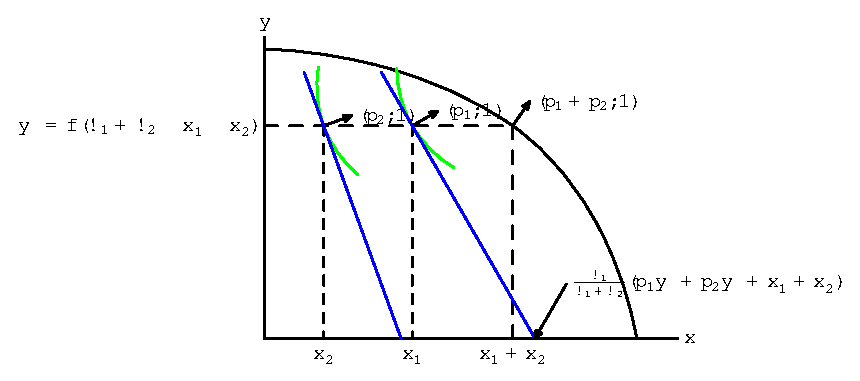
\includegraphics[width=4.9995in,height=2.3506in]{public_goods_fig8}
\par\end{center}

Notice that, when the firm increases production of the public good,
it receives revenue twice on each unit it produces. Consumer $1$
pays $p_{1}$ for that unit, but consumer $2$ also pays $p_{2}$
for it. So, the iso-profit curve for the profit maximizing firm that
must be tangent to the production possibilities frontier has slope
$\frac{1}{p_{1}+p_{2}}$. The firm earns its profits for its production
decision then distributes these profits to its owners. Consumer $1$
receives income 
\[
\frac{\omega_{1}}{\omega_{1}+\omega_{2}}\left(p_{1}y^{\ast}+p_{2}y^{\ast}+x_{1}^{\ast}+x_{2}^{\ast}\right)
\]
 which is labeled on the horizontal axis in Figure 4 . Consumer $2$
receives
\[
\frac{\omega_{2}}{\omega_{1}+\omega_{2}}\left(p_{1}y^{\ast}+p_{2}y^{\ast}+x_{1}^{\ast}+x_{2}^{\ast}\right)
\]
 which is the point where $2$'s budget line intersects the horizontal
axis (that has not been labeled in the figure to keep things simpler).

Consumer $1$ now faces a budget line (the blue line in the picture)
along which he chooses his best consumption bundle. Notice that since
consumer $1$ only buys good $y_{1}$ at price $p_{1}$ -- the slope
of this budget line is $\frac{1}{p_{1}}$ \emph{not} $\frac{1}{p_{1}+p_{2}}$.
So in this equilibrium, consumers marginal rates of substitution will
be different from the firm's marginal rate of substitution and generally
different from each other.

The market clearing conditions are twofold. First, consumers must
both choose to purchase the common level of output of the public good
that has been offered by the firm. Second, the sum of the private
good demand of each consumer must be equal to the total amount of
the private good that the firm has chosen to produce.

The prices that support this outcome are often know as Lindahl prices.
The reciprocal of the slope of the production possibilities frontier
is the marginal cost of producing one extra unit of the public good
(expressed in terms of units of the private good). Since the iso-profit
line must be tangent to the production possibilities curve, this marginal
cost is equal to $p_{1}+p_{2}$. The reciprocal of the slopes of the
consumers indifference curves are equal to their marginal willingness
to pay for the public good (again expressed in terms of the private
good). Since the indifference curves are tangent to the individual
budget lines, these willingnesses to pay are $p_{1}$ and $p_{2}$
respectively. So, the Lindahl prices ensure that the marginal cost
of producing the public good is exactly equal to the sum of the two
consumers' willingness to pay. 
\end{document}
